\definecolor{mygreen}{cmyk}{0.5,0,0.5,0.5}
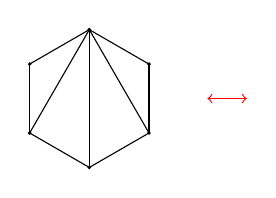
\begin{tikzpicture}[scale = .5]
		\tikzstyle{every node} = [font = \small]
		\foreach \x in {0}
		{
			\foreach \y in {-8}
			{
			\fill (\x,\y+1.75) circle (.05);
			%\fill (\x,\y+1.75) node [above] {\tiny{$1$}};
			\fill(\x+1.5158,\y+.875) circle (.05);
			%\fill (\x+1.5158,\y+.875) node [right] {\tiny{$2 $}};
			\fill (\x+1.5158,\y-.875) circle (.05);
			%\fill (\x+1.5158,\y-.875) node [right] {\tiny{$3$}};
			\fill(\x,\y-1.75) circle (.05);
			%\fill (\x,\y-1.75) node [below] {\tiny{$4$}};
			\fill(\x-1.5158,\y-.875) circle (.05);
			%\fill (\x-1.5158,\y-.875) node [left] {\tiny{$5$}};
			\fill (\x-1.5158,\y+.875) circle (.05);
			%\fill (\x-1.5158,\y+.875) node [left] {\tiny{$6$}};
		
			\draw [] (\x,\y+1.75)--(\x+1.5158,\y+.875); %v1 to v2
			\draw [] (\x+1.5158,\y+.875) -- (\x+1.5158,\y-.875); %v3 to v2
			\draw [] (\x+1.5158,\y-.875)--(\x,\y-1.75); %v4 to v3
			\draw [] (\x,\y-1.75) -- (\x-1.5158,\y-.875); %v5 to v4
			\draw [] (\x-1.5158,\y-.875)--(\x-1.5158,\y+.875); %v6 to v5
			\draw [] (\x-1.5158,\y+.875) -- (\x,\y+1.75); %v1 to v6
		
			\draw [] (\x,\y+1.75) -- (\x-1.5158,\y-.875);
			\draw [] (\x,\y+1.75) -- (\x,\y-1.75);
			\draw [] (\x,\y+1.75) -- (\x+1.5158,\y-.875);
		
			}
		}
		\draw[red,<->] (3,-8) -- (4,-8);
	\end{tikzpicture}
	\quad
	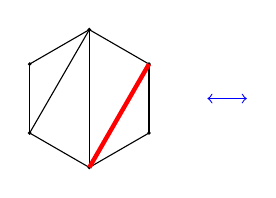
\begin{tikzpicture}[scale = .5]
		\tikzstyle{every node} = [font = \small]
		\foreach \x in {0}
		{
			\foreach \y in {-8}
			{
			\fill (\x,\y+1.75) circle (.05);
			%\fill (\x,\y+1.75) node [above] {\tiny{$1$}};
			\fill(\x+1.5158,\y+.875) circle (.05);
			%\fill (\x+1.5158,\y+.875) node [right] {\tiny{$2 $}};
			\fill (\x+1.5158,\y-.875) circle (.05);
			%\fill (\x+1.5158,\y-.875) node [right] {\tiny{$3$}};
			\fill(\x,\y-1.75) circle (.05);
			%\fill (\x,\y-1.75) node [below] {\tiny{$4$}};
			\fill(\x-1.5158,\y-.875) circle (.05);
			%\fill (\x-1.5158,\y-.875) node [left] {\tiny{$5$}};
			\fill (\x-1.5158,\y+.875) circle (.05);
			%\fill (\x-1.5158,\y+.875) node [left] {\tiny{$6$}};
		
			\draw [] (\x,\y+1.75)--(\x+1.5158,\y+.875); %v1 to v2
			\draw [] (\x+1.5158,\y+.875) -- (\x+1.5158,\y-.875); %v3 to v2
			\draw [] (\x+1.5158,\y-.875)--(\x,\y-1.75); %v4 to v3
			\draw [] (\x,\y-1.75) -- (\x-1.5158,\y-.875); %v5 to v4
			\draw [] (\x-1.5158,\y-.875)--(\x-1.5158,\y+.875); %v6 to v5
			\draw [] (\x-1.5158,\y+.875) -- (\x,\y+1.75); %v1 to v6
		
			\draw [] (\x,\y+1.75) -- (\x-1.5158,\y-.875);
			\draw [] (\x,\y+1.75) -- (\x,\y-1.75);
			\draw [red,ultra thick] (\x,\y-1.75) -- (\x+1.5158,\y+.875);
		
			}
		}
		\draw[blue, <->] (3,-8) -- (4,-8);
	\end{tikzpicture}
		\quad
	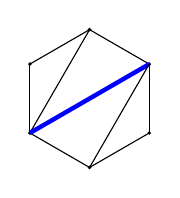
\begin{tikzpicture}[scale = .5]
		\tikzstyle{every node} = [font = \small]
		\foreach \x in {0}
		{
			\foreach \y in {-8}
			{
			\fill (\x,\y+1.75) circle (.05);
			%\fill (\x,\y+1.75) node [above] {\tiny{$1$}};
			\fill(\x+1.5158,\y+.875) circle (.05);
			%\fill (\x+1.5158,\y+.875) node [right] {\tiny{$2 $}};
			\fill (\x+1.5158,\y-.875) circle (.05);
			%\fill (\x+1.5158,\y-.875) node [right] {\tiny{$3$}};
			\fill(\x,\y-1.75) circle (.05);
			%\fill (\x,\y-1.75) node [below] {\tiny{$4$}};
			\fill(\x-1.5158,\y-.875) circle (.05);
			%\fill (\x-1.5158,\y-.875) node [left] {\tiny{$5$}};
			\fill (\x-1.5158,\y+.875) circle (.05);
			%\fill (\x-1.5158,\y+.875) node [left] {\tiny{$6$}};
		
			\draw [] (\x,\y+1.75)--(\x+1.5158,\y+.875); %v1 to v2
			\draw [] (\x+1.5158,\y+.875) -- (\x+1.5158,\y-.875); %v3 to v2
			\draw [] (\x+1.5158,\y-.875)--(\x,\y-1.75); %v4 to v3
			\draw [] (\x,\y-1.75) -- (\x-1.5158,\y-.875); %v5 to v4
			\draw [] (\x-1.5158,\y-.875)--(\x-1.5158,\y+.875); %v6 to v5
			\draw [] (\x-1.5158,\y+.875) -- (\x,\y+1.75); %v1 to v6
		
			\draw [] (\x,\y+1.75) -- (\x-1.5158,\y-.875);
			\draw [blue, ultra thick] (\x-1.5158,\y-.875) -- (\x+1.5158,\y+.875);
			\draw [] (\x,\y-1.75) -- (\x+1.5158,\y+.875);
		
			}
		}
	\end{tikzpicture}
	\quad \quad \quad \quad \quad \quad \quad \quad \quad \quad \quad
	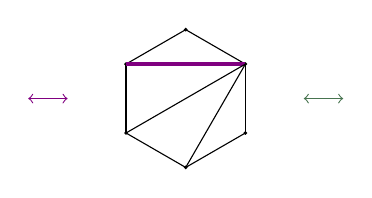
\begin{tikzpicture}[scale = .5]
		\tikzstyle{every node} = [font = \small]
		
		\draw[violet, <->] (-3,-8) -- (-4,-8);
		
		\foreach \x in {0}
		{
			\foreach \y in {-8}
			{
			\fill (\x,\y+1.75) circle (.05);
			%\fill (\x,\y+1.75) node [above] {\tiny{$1$}};
			\fill(\x+1.5158,\y+.875) circle (.05);
			%\fill (\x+1.5158,\y+.875) node [right] {\tiny{$2 $}};
			\fill (\x+1.5158,\y-.875) circle (.05);
			%\fill (\x+1.5158,\y-.875) node [right] {\tiny{$3$}};
			\fill(\x,\y-1.75) circle (.05);
			%\fill (\x,\y-1.75) node [below] {\tiny{$4$}};
			\fill(\x-1.5158,\y-.875) circle (.05);
			%\fill (\x-1.5158,\y-.875) node [left] {\tiny{$5$}};
			\fill (\x-1.5158,\y+.875) circle (.05);
			%\fill (\x-1.5158,\y+.875) node [left] {\tiny{$6$}};
		
			\draw [] (\x,\y+1.75)--(\x+1.5158,\y+.875); %v1 to v2
			\draw [] (\x+1.5158,\y+.875) -- (\x+1.5158,\y-.875); %v3 to v2
			\draw [] (\x+1.5158,\y-.875)--(\x,\y-1.75); %v4 to v3
			\draw [] (\x,\y-1.75) -- (\x-1.5158,\y-.875); %v5 to v4
			\draw [] (\x-1.5158,\y-.875)--(\x-1.5158,\y+.875); %v6 to v5
			\draw [] (\x-1.5158,\y+.875) -- (\x,\y+1.75); %v1 to v6
		
			\draw [violet, ultra thick] (\x-1.5158,\y+.875) -- (\x+1.5158,\y+.875);
			\draw [] (\x-1.5158,\y-.875) -- (\x+1.5158,\y+.875);
			\draw [] (\x,\y-1.75) -- (\x+1.5158,\y+.875);
		
			}
		}
		\draw[mygreen, <->] (3,-8) -- (4,-8);
	\end{tikzpicture}
		\quad
	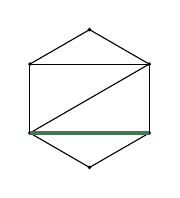
\begin{tikzpicture}[scale = .5]
		\tikzstyle{every node} = [font = \small]
		\foreach \x in {0}
		{
			\foreach \y in {-8}
			{
			\fill (\x,\y+1.75) circle (.05);
			%\fill (\x,\y+1.75) node [above] {\tiny{$1$}};
			\fill(\x+1.5158,\y+.875) circle (.05);
			%\fill (\x+1.5158,\y+.875) node [right] {\tiny{$2 $}};
			\fill (\x+1.5158,\y-.875) circle (.05);
			%\fill (\x+1.5158,\y-.875) node [right] {\tiny{$3$}};
			\fill(\x,\y-1.75) circle (.05);
			%\fill (\x,\y-1.75) node [below] {\tiny{$4$}};
			\fill(\x-1.5158,\y-.875) circle (.05);
            %\fill (\x-1.5158,\y-.875) node [left] {\tiny{$5$}};
			\fill (\x-1.5158,\y+.875) circle (.05);
			%\fill (\x-1.5158,\y+.875) node [left] {\tiny{$6$}};
		
			\draw [] (\x,\y+1.75)--(\x+1.5158,\y+.875); %v1 to v2
			\draw [] (\x+1.5158,\y+.875) -- (\x+1.5158,\y-.875); %v3 to v2
			\draw [] (\x+1.5158,\y-.875)--(\x,\y-1.75); %v4 to v3
			\draw [] (\x,\y-1.75) -- (\x-1.5158,\y-.875); %v5 to v4
			\draw [] (\x-1.5158,\y-.875)--(\x-1.5158,\y+.875); %v6 to v5
			\draw [] (\x-1.5158,\y+.875) -- (\x,\y+1.75); %v1 to v6
		
			\draw [] (\x-1.5158,\y+.875) -- (\x+1.5158,\y+.875);
			\draw [] (\x-1.5158,\y-.875) -- (\x+1.5158,\y+.875);
			\draw [mygreen, ultra thick] (\x-1.5158,\y-.875) -- (\x+1.5158,\y-.875);
		
			}
		}
	\end{tikzpicture}